\documentclass[a4paper,twoside,kulak]{kulakreport} %options: kul or kulak (default)

\usepackage[dutch]{babel}
\usepackage{pdfpages}

\faculty{Wetenschap \& Technologie Kulak}
\group{Ingenieurswetenschappen}
\title{Smart city}
\subtitle{Tussentijds verslag}
\author{Groep 6}
\institute{Aaron Vandenberghe, Dieter Demuynck, Mathis Bossuyt, Rani Jans, Sarah De Meester, Jolien Barbier}
\date{Academiejaar 2020 -- 2021}
\address{
   KU Leuven Kulak           \\
   Wetenschap \& Technologie \\
   Etienne Sabbelaan 53, 8500 Kortrijk             \\
   Tel.\ +32 56 24 60 20     \\
  
   }


\begin{document} % hier begint de eigenlijke inhoud van het document
%Wat allemaal in het doc verwerkt moet zitten:
%-klantenvereisten
%-ontwerpsspecificaties
%-ontwerpskeuze
%-financieel rapprot
%-evaluatie wat gedaan is en wat nog moet gebeuren en hoe
%-wat nog verbeterd kan worden aan ontwerp

\titlepage

\tableofcontents
\renewcommand\thesection{\arabic{section}}
\renewcommand\thesubsection{\thesection.\arabic{subsection}}
\newpage
\section*{Inleiding}
%probleemstelling
%Ontwerpsproces en planning

Bij het ontwerpen van een zelfrijdend wagentje komt er heel wat bij te kijken. Wat houdt het project in? Het wagentje moet in staat zijn zich volgens een voorgeprogrammeerde route door een modelstad te bewegen. Dit is het idee van de 'Smart City'. 'Smart city', ook wel 'Slimme Stad' genoemd, is een stad waarbij informatietechnologie gebruikt wordt om de stad te beheren en te besturen \cite{SmartCity}. Doorheen deze route, komt het wagentje verschillende obstakels tegen. De bedoeling is dat deze worden herkend en dat er een bijpassende actie wordt uitgevoerd. Hoe dit kan worden geïmplementeerd zal aan bod komen in dit verslag.
Dit verslag zal een beeld geven van hoe dit project moet aangepakt worden. Het ontwerpproces wordt uitvoerig uitgelegd. Hierin wordt het aanschaffen van onderdelen en de vereisten toegelicht. Hoe men te werk gaat op vlak van planning wordt ook toegelicht.

\section{Ontwerpproces}

\subsection{Onderdelen}

%Wat auto moet kunnen en algemeen wat je zal gebruiken.
Eerst en vooral is het belangrijk om een idee te krijgen over alle cruciale onderdelen die zullen gebruikt worden in het project. 

Een van de basisonderdelen is de chassis. Op dit onderdeel zal alles worden gemonteerd. Het is als het ware de ruggengraat van de auto.%wikipedia chassis
Opdat de auto kan rijden zijn uiteraard wielen nodig. In het model dat verder wordt beschreven, worden er twee reguliere ronde wielen gebruikt en één ball caster. Om de aandrijving van de wielen mogelijk te maken wordt er aan ieder rond wiel een microtandwielmotor geplaatst. De regeling van de motoren gebeurt via de dual drive motor. Om uiteindelijk geheel de auto te laten voortbewegen is er een nood aan een hardwarecomponent namelijk een microcontroller. Deze fungeert als een soort mini computer. Daarnaast zal ook extra stroomtoevoer moeten worden voorzien. Hiervoor worden twee oplaadbare lithium-ion batterijen gebruikt. Verder is het ook nuttig om gebruik te maken van een breadboard. Dit is echter geen onderdeel van de zelfrijdende auto, maar is handig voor het testen van elektrische circuits.

\subsection{Vereisten} %aanpassing woord!!
% Wat moet de auto  kunnen
De auto moet over het algemeen lijnen herkennen en deze volgen, stoppen bij een rood licht, andere wagens detecteren en stoppen als de auto te dicht bij een voorligger komt. Men moet ook van op afstand kunnen ingrijpen.

Nadat het wagentje de lijn herkent, moet hij deze kunnen interpreteren. Er wordt namelijk een onderscheid gemaakt tussen twee soorten lijnen: volglijnen en stoplijnen. Het verschil tussen deze twee lijnen zit hem in de dikte. Volglijnen zijn 25 mm dik, stoplijnen 50 mm. De wagen zal dus de lijnen van 25 mm dik moeten volgen en moeten stoppen bij de lijnen van 50 mm dik. De wagen moet dus een sensor bevatten deze lijnen kan herkennen, meer bepaald een reflectiesensor. Deze zal onderaan het wagentje geplaatst worden zodat de lijnen makkelijk worden herkend.

De wagen komt een stoplijn tegen bij het naderen van een kruispunt. Hier zal hij moeten tot stilstand komen en een verkeerslicht moeten interpreteren. Het wagentje zal dus moeten voorzien zijn van een kleurensensor of een camera die de twee verschillende kleuren van het stoplicht kan onderscheiden. Bij een rood licht zal hij moeten stoppen aan de stoplijn, bij groen zal hij weer mogen starten.

Ook moet het wagentje voorgaande wagens kunnen detecteren en stoppen wanneer deze te dichtbij komen. Als de wagen van achter wordt aangereden is dit niet zijn fout, dus enkel voorliggers kunnen een probleem vormen. Om andere wagens te herkennen moet het wagentje een afstandssensor bevatten die voorliggers detecteert en vervolgens een signaal verzendt zodat de motoren vertragen om een botsing te voorkomen. Er moet dus ook gezorgd worden een zo kort mogelijke remafstand.

Verder moet het wagentje aan een aanvaardbare snelheid voortbewegen. De micro tandwielmotoren rond de wielen zorgen voor de aandrijving. Daarbij is het belangrijk dat het wagentje een beperkte massa heeft, maximaal 500 gram. Dit zal ervoor zorgen dat het wagentje op een veilige manier zich aan ongeveer 10 cm/s kan voortbewegen zodat ook de remafstand beperkt blijft.

Ten slotte moet men vanop afstand kunnen ingrijpen wanneer er iets fout loopt.


%Per onnderdeel verwijzen voor bibliografie!!!

%- herkennen lijnen: welke soort sensor (bv reflectie voor lijnen)
%- stoplicht: kleurensensor, tot stilstand komen blabla
%- snelheid: massa belangrijk
%- andere wagens detecteren => remafstand, massa belangrijk => stoppen door signaal zodat motoren vertragen
%- op afstand ingrijpen


\subsection{Ontwerpskeuze}
%Zeer specifiek toelichten waarom je elk onderdeel heb gekozen.

In deze sectie wordt aanvullende uitleg gegeven over elk onderdeel dat in het project wordt gebruikt. Daarnaast wordt extra beargumenteerd waarom dit specifiek onderdeel is gekozen.

\subsubsection{Chassis}
Als eerste wordt de chassis gesproken. Voor deze auto wordt een rechthoekige chassis gebruikt met als afmetingen 80 mm op 172 mm zoals kan gevonden worden op site \cite{RobotChassisRechthoekigZwart}. %verwijzing chassis materiaal
Deze chassis is zeer handig in gebruik wegens de verscheidene groottes van de groeven. Bovendien is de rechthoekige vorm zeer gemakkelijk om alle componenten van de auto vast te hechten. Een ronde chassis zoals bijvoorbeeld van de site \cite{RobotChassis} is hiervoor minder geschikt. Ook zijn er in deze laatste groeven aanwezig voor de wielen. Dit impliceert dat er minder ruimte is om andere onderdelen te assembleren op het onderstel. 

~
\subsubsection{Wielen}
Een goede keuze voor wielen zijn deze met respectievelijk een diameter en dikte van 42 mm en 19 mm. De site \cite{Wiel42x19mm} geeft een idee hoe het wiel eruit ziet. De dikte van dit wiel is echter geschikt om voldoende grip te hebben. Dit is minder bij dunnere wielen waardoor dit niet ideaal is voor dit model. Daarnaast zorgt de grootte van de diameter voor een relatieve grote versnelling en een gemiddelde kracht. Een kleiner wiel impliceert namelijk een kleinere kracht en een kleine versnelling. Een groot wiel daarentegen levert een grote versnelling maar heeft een grote kracht nodig. Het is dus belangrijk dat de middenweg wordt genomen om een goede snelheid te behalen zonder al te veel moeite. Dit kan perfect met wielen van de grootte zoals hierboven aangegeven. 

Zoals eerder aangegeven is de auto van dit project een driewieler. Dit heeft enkele voordelen. Eerst en vooral is dit eenvoudiger om manoeuvres zoals draaien te voltooien. Ten tweede reduceert een driewieler de kosten van het project. Idealiter wordt als derde wiel gebruik gemaakt van een ball caster. Op die manier moet er geen extra tandwielmotor en bijhorende zaken zoals een tandwielmotorsbeugel worden aangekocht. Daarnaast beperkt dit ook het extra gewicht op de auto waardoor het zou kunnen vertragen.

~

\subsubsection{Motoren}
Aansluitend hierbij spelen de tandwielmotoren hier ook een belangrijke rol bij. Motoren met een groot tandwiel starten zeer gemakkelijk maar behalen geen al te grote snelheid. Kleine tandwielen hebben dan weer de omgekeerde eigenschap. Het is dus weer van belang dat er een tandwielen worden gebruikt met een gemiddelde grootte namelijk de motor met de verhouding 50:1. Niet alleen de grootte speelt een rol bij de tandwielmotoren, maar ook de kracht van de motor. Hiervoor wordt het best gekozen voor de "High Power" (HP). Deze motoren hebben een grotere efficiëntie. Een bijkomend voordeel is het gewicht dat slechts 9,5 gram bedraagt \cite{MicroMetalGearMotor50:1HP}. %Erbij zetten dat het ook een groter vermogen heeft?

Het is vanzelfsprekend dat door het gebruik van deze tandwielen nood is per motor aan een tandwielmotorbeugel opdat de tandwielmotoren aan de chassis kunnen vast gemaakt worden. Aangezien de motoren een breedte van 12 mm hebben en een hoogte van 10 mm als diameter hebben, heeft het als logisch gevolg dat de beugel met lengtes 12 mm op 10 mm worden genomen \cite{MicroMetalGearMotorBeugel}.
Verder is een dual drive motor essentieel om de tandwielmotoren met de microcontroller te verbinden. In dit project wordt gekozen voor de Dual Drive DRV8833 \cite{DualDriveDRV8833}. %site vermelden


~
\subsubsection{Microcontroller}
Volgend component is cruciaal voor de werking van de auto. Zoals eerder vermeld zorgt de microcontroller er immers voor dat het autootje de taken correct uitvoert. Dit keuze van de microcontroller gaat in dit project naar NI MyRIO in plaats van Raspberry Pi. Dit heeft enkele gevolgen. 
Eerst en vooral hebben de inputs de mogelijkheid om een digitaal of een analoog signaal door te geven. Bij Raspberry Pi zijn er enkel digitale inputs beschikbaar. Dit heeft implicaties voor de keuze van de sensoren. Ten tweede zal alles in LabVIEW worden geprogrammeerd. Deze software en microcontroller zijn ervoor gemaakt om samen te werken. Dit biedt veel voordelen tijdens de implementatie. %site van de microcontroller

~
\subsubsection{Sensoren}
Zoals al aangehaald is, wordt in dit ontwerp gewerkt met een reflectiesensor en een afstandssensor. Er bestaan 2 soorten, namelijk sensoren met digitale output en met analoge output. Beide kunnen gebruikt worden met de NI MyRIO. De analoge sensoren geven meer info dan de digitale. De digitale kunnen maar één of twee signalen doorgeven aan de microcontroller namelijk nul of een. Ofwel staat de sensor aan ofwel uit. De analoge sensoren geven daartegenover een nauwkeurige feedback en echte waarden. Langs de andere kant zorgen de analoge sensoren voor meer programmeerwerk \cite{DigitaalOfAnaloog}. Voor dit project is het beter dat de informatieoverdracht tussen sensor en microcontroller vlot verloopt met behulp van echte waarden. Bij keuze van een analoge sensor is dit dus voldaan, alhoewel er meer programmeerwerk bij komt kijken. %echte waarden nog wat uitleggen wat ermee bedoeld wordt.

~

Ook om kleuren te herkennen, is er nood aan een sensor of camera. We hadden de keuze tussen een RPi camera, webcam en kleurensensor voor het interpreteren van de stoplichten. In dit ontwerp wordt er niet voor gekozen om de camera en webcam te gebruiken. De webcam weegt namelijk 223,6 gram terwijl de kleurensensor 3,23 gram weegt \cite{Webcam,TCS34725KleurSensorBOB}. Hoe minder de wagen weegt, hoe stabieler het is en hoe minder kracht het nodig heeft om een bepaalde snelheid te kunnen halen. Bovendien is de camera enkel bruikbaar is met een Raspberry Pi als microcontroller. Aangezien in dit model wordt gewerkt met een NI MyRIO, is dit dus geen optie \cite{RPi-camera}. Samengevat: de kleurensensor heeft dus als voordeel dat het zeer licht is en compatibel is met de NI MyRIO als microcontroller.

~

\subsubsection{LED-lampjes}
We kozen als optie om LED's te plaatsen omdat het ons het meest haalbaar leek in vergelijking met de andere ideeën. Eerst dachten we eraan om servomotoren te gebruiken maar deze waren schaars en ingewikkeld te modelleren waardoor er risico zou zijn dat het wagentje niet juist werkt.
%Gear-motor: niet 100, want anders veel toeren, maar te weinig kracht (50 omgekeerd)

\subsection{Assemblage}
%titel nog aan te passen
%Alles op elkaar zetten, 3D-modellen?
%NOG DOEN


\subsection{Implementatie}
%titel nog aan te passen


Om te kunnen implementeren is men eerst en vooral bezig geweest met opzoekwerk. Vanaf week 1 is het best om te weten welke sensoren, motoren en microcontrollers nodig zijn. Vanaf week 3 moet er specifieker gezocht worden hoe het materiaal best gebruikt kan worden. 
%bron myrio nog vermelden
Dit deed men om de communicatie tussen de sensoren en de NI MyRIO-controller te begrijpen. Ook het aantal volt dat nodig is om de sensoren te laten te werken is belangrijk. Zo zijn er een paar poorten waar er precies 5 volt uitkomt ,wat perfect is voor de sensoren omdat deze 5 volt nodig hebben om te kunnen werken. Eens dit geweten is, begint men met het elektrisch circuit op te stellen. Dit is handig om te weten welke onderdelen er met elkaar worden verbonden. Eens dit in orde is, kan het programmeerwerk beginnen.

Het schrijven van stukjes code begon pas echt in week 6. Dit was zo omdat we het materiaal dan voor ons hadden liggen en onze stukjes code effectief konden testen. Met de eerste test probeerden we de lampjes op de microcontroller te laten branden. Dit deden we via de 'LED' functie van LabVIEW. Onze tweede test was het versturen en ontvangen van signalen. Het programma \texttt{main.vi} dat standaard in LabVIEW onder myrio staat heeft weer hoe de microcontroller beweegt. We hebben dit standaard programma gebruikt bij onze testen. We hebben op de controller een draad bevestigd tussen poort 11A en 13A. Op het moment dat het kantelt en op de z-as meer dan 0.5 wordt weergegeven moet het via 11A een signaal versturen. Dit werd dan ontvangen door 13A. Als 13A een signaal kreeg moest de controller een signaal sturen naar de computer waardoor een bol groen kleurt. 

Het echt programma zal bestaan uit verschillende subVI's. Zo zullen we een stukje code schrijven dat specifiek is voor het detecteren van wagens die voor ons rijden. Als er een obstakel minder dan 20 cm voor ons staat zal hij moeten stoppen of de snelheid aanpassen. Een ander stukje code zal het lezen van het stoplicht zijn. Hier zal de microcontroller de signalen van kleursensor moeten interpreteren. Een ander deel zal met de reflectie sensor de volglijn volgen en weten wanneer die overgaat in een stopstreep waarna het wagentje moet stoppen.
Er zal ook een deel zijn over het kruispunt. Dit zal bestaan uit 3 delen. Deze zijn rechtdoor rijden en links of rechts afslaan. Hieraan zullen de richtingsaanwijzers gekoppeld worden. 

\subsubsection{Experimenten}

We experimenteren met de sensoren. Voorbeeldprogramma's worden gemaakt om de data die we krijgen van de sensoren te interpreteren. Op die manier weten we met welke waarden we moeten werken in ons echt programma. 

Het eerste experiment met sensoren was met de reflectiesensor. Dat is een programma dat de 6 waarden van de sensor weer geeft. Omdat het miniatuur robotwagentje helder en donker moet onderscheiden hebben we die getest op wit papier waarbij we waarden rond de 1 krijgen. Om de waarden bij van het donkere spectrum te krijgen, hebben we het zwart van de laptop gebruikt. Hier kregen we waarden rond de 4 tot 4.5. We hebben het ook gedaan op de grijze tafels.
Nu gaan we die waarden gebruiken om te weten wat de lijn is die we zullen moeten volgen.
We hebben het aantal waarden dat we krijgen per seconde wat vermindert van 1000 naar 100 om op die manier stabielere inputs te krijgen. Anders was het moeilijk om die waarden te lezen.


De volgende test was met de afstandssensor. Als de afstand tussen de sensor en het voorwerp groot is krijgen we lage waarden (ongeveer 0.1). Als er binnen de 80 cm niets staat dan worden de waarden negatief. Dit stijgt tot een maximale waarde van 3 bij ongeveer 10 cm. Als we het object dichter dan 10 cm houden dan zakt de waarde die we van de sensor krijgen naar 2. We weten nu dat we waarden tussen de 2 en 3 gaan moeten gebruiken. 

\section{Planning}
%Eerst hebben we nagedacht over welke materialen we nodig zullen hebben. Daarvoor is het best om vooral veel opzoekingswerk te doen om meer te weten te komen over de materialen. Het was vooral belangrijk om na te gaan welke onderdelen samengaan en welke niet. Dan wogen we af welke opties we hebben. Voor de aankoop van de materialen maakten we twee alternatieve modellen.

%Om zo efficiënt mogelijk te werken, verdeelden we onze groep in twee zodat één deel volop kon werken aan het implementeren in LabVIEW terwijl het andere deel de CAD-modellen en technische tekeningen in orde brachten.


%De CAD-modellen en technische tekeningen worden gebruikt om meer inzicht te krijgen in hoe het wagentje eruit zal zien.

%wat hebben we tot nu kunnen bereiken
%hoe kunnen we ons ontwerp nog verbeteren
%experimenten met LabVIEW 



%Eerst bestelden we onze materialen. Van deze hebben we CAD-modellen en technische tekeningen gemaakt om inzicht te krijgen in de opbouw. We zijn voorlopig nog bezig met de implementatie en de assemblage van het wagentje.


Om te beginnen aan dit soort project, is het noodzakelijk om eerst op lange termijn te plannen: algemeen van welke 'grote' taken moeten er na een bepaalde tijd zeker afgewerkt zijn. Eerst en vooral moeten een aantal technische aspecten in orde zijn voordat we echt van werk kunnen gaan. Het aanmaken van een stuklijst is noodzakelijk om een beeld te krijgen van hoeveel we ongeveer zullen besteden rekening houdend met het budget. Hierbij is het ook zeer belangrijk om na te gaan welke onderdelen samen gaan en welke niet om fouten zoals bijvoorbeeld het bestellen van een motorbeugel die niet op de motor past te vermijden.

Nadat de onderdelen met behulp van de stuklijst worden besteld, kan men praktisch aan de slag gaan met de sensoren, motoren en microcontroller om deze te implementeren in LabVIEW. Hoe men hieraan te werk is gegaan wordt beschreven in sectie 0.1.5.

Verder worden er 3D-modellen van de onderdelen met behulp van Solid Edge gemaakt. Dit geeft ons een beter beeld van hoe het wagentje eruit zal zien. Hierbij horen ook de technische tekeningen. Deze zijn handig bij het opzoeken van afmetingen van de aparte onderdelen. Als alle 3D-modellen in orde zijn, kan er gestart worden met de assemblage. Dit is een 3D-voorstelling in Solid Edge waarbij alle onderdelen als het ware aan elkaar worden geplakt. Als de assemblage in Solid Edge compleet is, kan er beslist worden welke mechanische stukken zoals MakerBeams er zullen passen op de wagen.


\section{Bijlagen}
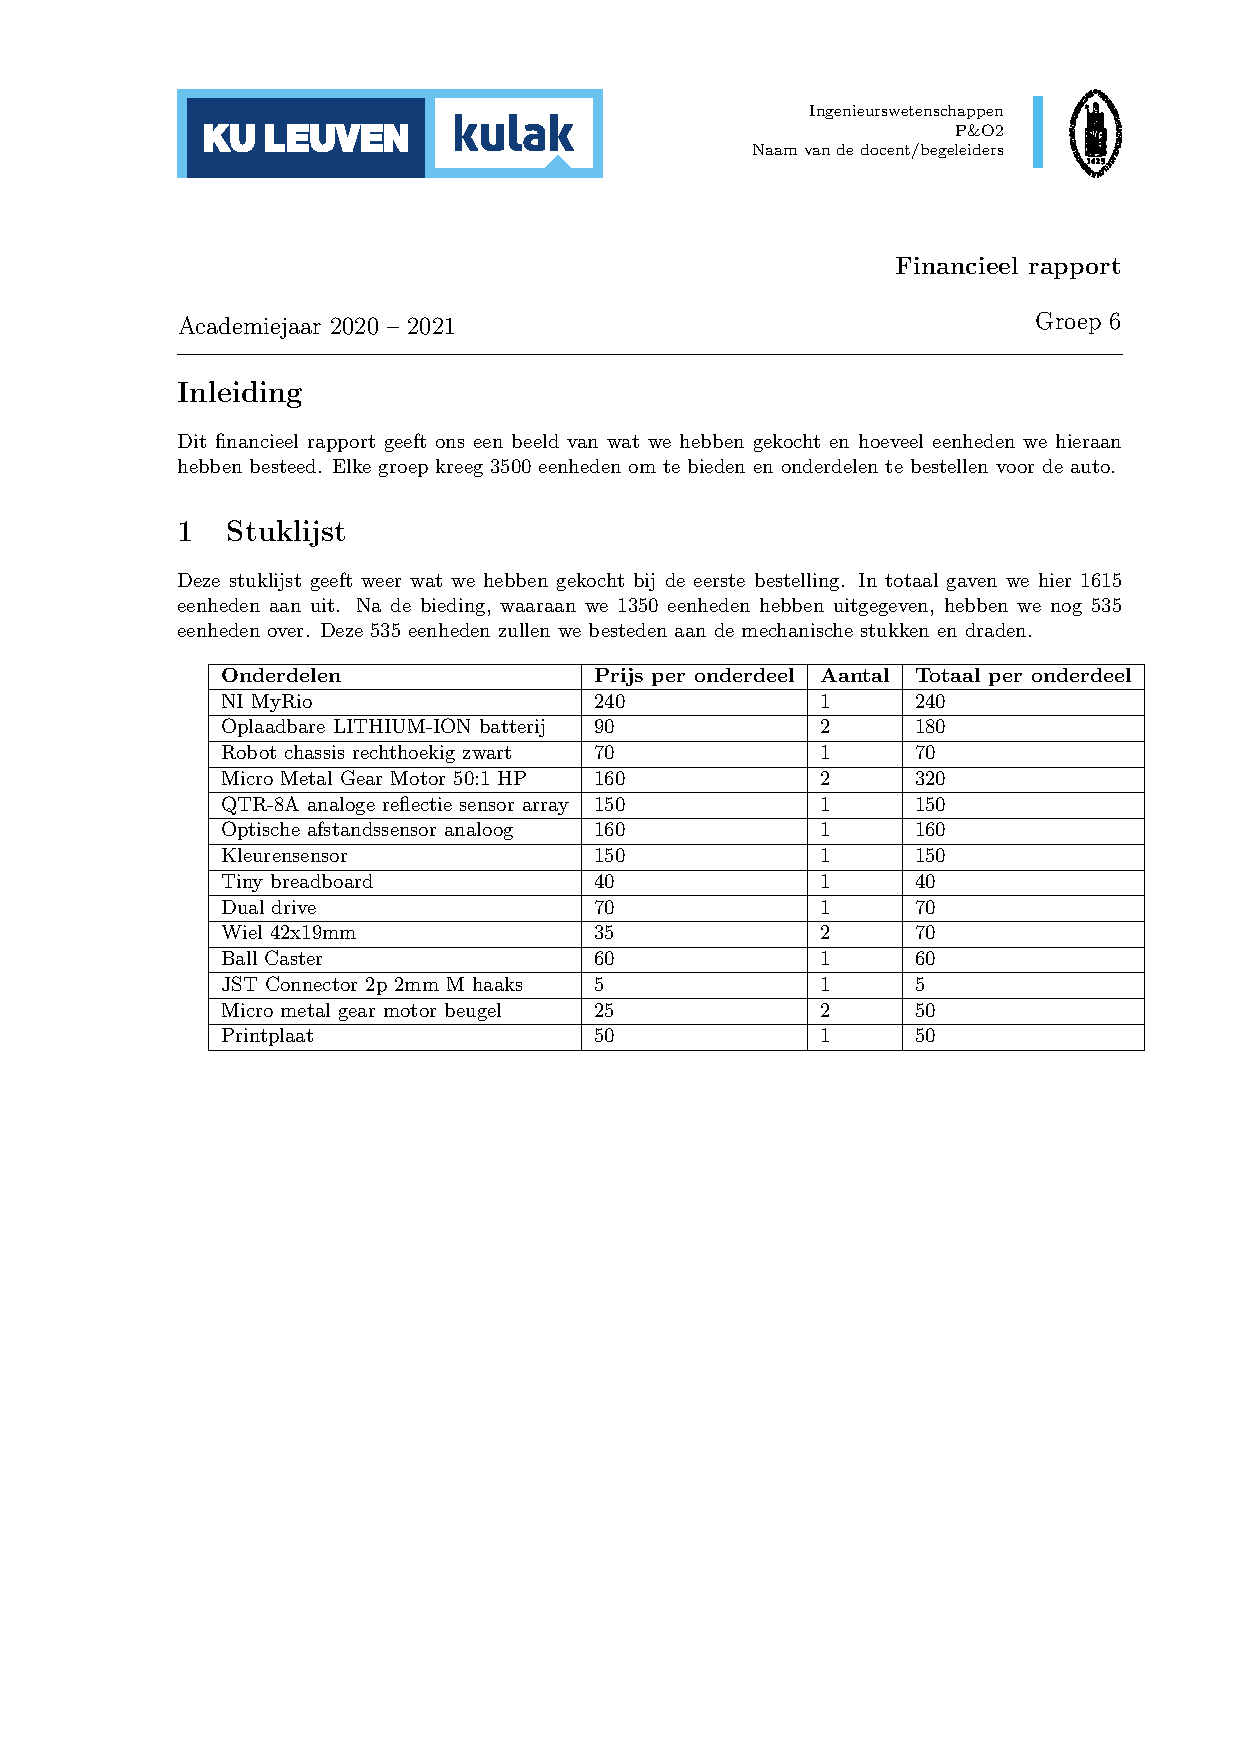
\includepdf{FinancieelRapport.pdf}


\chapter*{Besluit}
Afsluitende tekst.

\bibliographystyle{plain}
\bibliography{bronnen_verslag}
\bibliographystyle{unsrt}
\end{document}
